\documentclass[11pt]{article} 

\usepackage{geometry} 
\geometry{a4paper} 

\usepackage{graphicx}


\title{Studio di un modello predittivo del periodo di oscillazione di un pendolo fisico}
\author{Francesco Angelo Fabiano Antonacci\\Alessandro Di Meglio}
\date{\today} 
\begin{document}
\maketitle

\section{Scopo dell'esperienza}

In questa relazione di laboratorio si intende verificare sperimentalmente il modello predittivo del periodo di un pendolo fisico dato dall'equazione $T(d)=2\pi\sqrt{\frac{\frac{l^2}{12}+d^2}{gd}}$.

\section{Cenni teorici}

Un corpo rigido sospeso in un punto diverso dal centro di massa e sottoposto all' accelerazione di gravità costituisce un pendolo fisico.
\begin{figure}[htbp]
\centerline{\includegraphics[width=6cm, height=6cm]{physicalpendulum_image.png}}

\label{fig}
\end{figure}

Se spostato di un angolo $\theta$ dalla posizione di equilibrio, il momento torcente agente sul corpo rispetto al centro in cui è incernierato è fornito dalla seguente equazione:
\begin{equation}
\tau  = -mgd sin(\theta)
\end{equation}

Per la seconda equazione cardinale si ha anche che:


\begin{equation}
\tau  =\frac{dL}{dt}
\end{equation}

Per le relazioni $L=I\omega  $ e $\omega=\frac{d\theta}{dt}$, è  possibile ottenere la seguente equazione:

\begin{equation}
\tau=I\frac{d\theta^2}{dt^2}
\end{equation}
Combinando la (1) e la (3) otteniamo:
\begin{equation}
I\frac{d\theta^2}{dt^2}+\frac{mgd}{I}sin(\theta)=0
\end{equation}
Quest'equazione differenziale, con le dovute considerazioni discusse nella sezione "\textbf{Piccole Oscillazioni}",
è approssimabile con quella del moto armonico con $T_0=2\pi\sqrt{\frac{I}{mgd}}$ .

Con le dovute considerazioni discusse nella sezione "\textbf {Approssimazioni}", consideremo il momento di inerzia del corpo rispetto all'asse perpendicolare all'asse dell'asta passante per il centro di massa come $I_{cm}=\frac{ml^2}{12}$.

Per il teorema di Huygens-Steiner I in un generico asse parallelo a quello appena considerato sarà $I=\frac{ml^2}{12}+d^2m$.
Da cui otteniamo, ponendola a sistema con le precedenti, l'equazione che costituisce il modello predittivo del periodo che si intende verificare:

\begin{equation}
T(d)=2\pi\sqrt{\frac{\frac{l^2}{12}+d^2}{gd}}
\end{equation}

\section{Apparato sperimentale}
\subsection{Asta Forata}
L'oggetto che costituisce il pendolo fisico in questo esperimento è un'asta di allumino.
Lungo l'asta vi è successione di fori identici ed equidistanti.
Le seguenti misure sono state prese col metro a nastro, eccetto quella dei diametri dei fori la quale è  stata effettata con il calibro ventesimale.
Si riportano le misure delle dimensioni dell'asta in "Table1", quelle del diametro e della distanza dei fori in "Table2".
\begin{table}
\centering

\caption{Misure dell'asta}
\begin{tabular}[t]{|c|c|c|}
 Lunghezza asta &Spessore1&Spessore2\\
  \hline
  $1.050 \pm 0.001$ m & $0.015 \pm 0.001$ m & $0.015 \pm 0.001$ m \\
\end{tabular}

\end{table}


\begin{table}
    \centering
\caption{Diametro dei fori e rispettiva distanza dei centri da un estremo dell'asta}
    \label{tab:lunghezza-asta}
    \begin{tabular}{|c|c|}
        \hline
        Diametro & Distanza\\
        \hline
         $0.005 \pm 0.0005$m & $0.050 \pm 0.001$ m \\
        $0.005 \pm 0.0005$m & $0.150 \pm 0.001$ m \\
        $0.005 \pm 0.0005$m & $0.250\pm 0.001$ m \\
        $0.005 \pm 0.0005$m & $0.350 \pm 0.001$ m \\
        $0.005 \pm 0.0005$m & $0.450 \pm 0.001$ m \\
        $0.005 \pm 0.0005$m  & $0.550 \pm 0.001$ m \\
        $0.005 \pm 0.0005$m & $0.650 \pm 0.001$ m \\
       $0.005 \pm 0.0005$m & $0.750 \pm 0.001$ m \\
       $0.005 \pm 0.0005$m & $0.850 \pm 0.001$ m \\
        $0.005 \pm 0.0005$m & $0.950 \pm 0.001$ m \\
        \hline
    \end{tabular}
\end{table}

\subsection{Supporto}
L'asta è stata incernierata alla parte terminale di un supporto, consistente in una barra metellica disposta parallela al terreno. 
Il vincolo della cerniera era una vite passante per i fori dell'asta e poggiante su cuscinetti a sfera per ridurre l'attrito durante il movimento.
Nella sezione "\textbf{Approssimazioni}"  si discute il comportamento del supporto durante l'esperimento.


\subsection{Strumenti di misura}
\begin{enumerate}
\item Cronometro digitale con risoluzione di un centesimo di secondo.
\item Metro a nastro con risoluzione di un millimetro.
\item Calibro con risoluzione di un ventesimo di millimetro.

\end{enumerate}
\section{Descrizione delle misure}

Riportiamo i dati ottenuti dalle misure  di 5 periodi  a "Table3"

\begin{table}
    \centering
    \caption{Misure di 5 periodi iterate 10 volte per ciascuno dei 10 fori. Vedi "\textbf {Errori di misura sui periodi misurati}"}
 
    \begin{tabular}{|c|c|c|c|c|c|c|c|c|c|}
        \hline
        \textbf{F1} & \textbf{F2} & \textbf{F3} & \textbf{F4} & \textbf{F5} & \textbf{F6} & \textbf{F7} & \textbf{F8} & \textbf{F9} & \textbf{F10} \\
        \hline
 
  8.04 & 7.85 & 7.80 & 8.37 & 11.40 & 19.01 & 9.29 & 7.99 & 7.80 & 7.94 \\
  8.35 & 7.89 & 7.85 & 8.44 & 11.29 & 18.91 & 9.29 & 8.09 & 7.91 & 7.98 \\
  8.04 & 7.92 & 7.80 & 8.37 & 11.35 & 18.76 & 9.24 & 8.01 & 7.86 & 8.04 \\
  8.19 & 7.84 & 7.77 & 8.42 & 11.40 & 18.97 & 9.50 & 8.05 & 7.77 & 8.06 \\
  8.13 & 7.91 & 7.86 & 8.32 & 11.54 & 19.00 & 9.35 & 7.97 & 7.79 & 8.17 \\
  8.13 & 7.78 & 7.92 & 8.38 & 11.35 & 19.04 & 9.30 & 8.04 & 7.83 & 7.92 \\.
  8.13 & 7.85 & 7.76 & 8.22 & 11.41 & 18.84 & 9.36 & 7.99 & 7.87 & 7.96 \\
  8.18 & 7.96 & 7.79 & 8.30 & 11.48 & 18.85 & 9.31 & 8.04 & 7.86 & 7.91 \\
  8.16 & 7.99 & 7.84 & 8.31 & 11.40 & 18.92 & 9.37 & 7.98 & 7.83 & 8.10 \\
  8.17 & 7.99 & 7.86 & 8.26 & 11.39 & 18.66 & 9.29 & 8.03 & 7.90 & 8.11 \\
 \hline
    \end{tabular}
   \caption{}
\end{table}


\subsection{Errori di misura sui periodi misurati}
Per le misure di tempo è stato usato un cronometro. Per calcolare l'incertezza è stato necessario valutare i tempi di reazione degli sperimentatori: fatti partire due cronometri nello stesso istante, uno sperimentatore ha interrotto il proprio cronometro non appena ha visto l'altro interrompere il proprio. Lo scarto delle misure è stato considerato l'errore dovuto al tempo di reazione.
Rappresentiamo la formula che descrive l'incertezza che abbiamo misurato per i periodi:
\begin{equation}
\sigma_T=\sqrt{tempo_{strumento}^2 + tempo_{reazione}^2}
\end{equation}



\begin{table} 
\centering
\begin{tabular}{|c|c|}
 
\hline
  Tempo di reazione & Risoluzione Strumentale \\
  \hline
  $0.27 $ s & $0.01$ s \\
  $0.15$ s & $0.01$ s \\
  $0.21$ s & $0.01$ s \\
  $0.23$ s & $0.01$ s \\
  $0.16$ s & $0.01$ s \\
  \hline

\end{tabular}
\end{table}




\subsection{Errori di misura sulle lunghezze}
E' stata assunta come incertezza delle misure prese col metro a nastro la risoluzione dello strumento: $\sigma l_{metro}=0.001 m$.
E' stata assunta come incertezza delle misure prese col calibro ventesimale la risoluzione dello strumento $\sigma l_{calibro}=0.0005 m$.
\subsection{Approssimazioni}
\subsubsection{Supporto}
E' stato osservato che nonostante il supporto del particolare esperimento fosse potenzialmente soggetto ad oscillazioni in tutti i gradi di libertà per effetti di elasticità, nelle particolari sollecitazioni dell'esperimento è ragionevole supporlo come immobile.
\subsubsection{Momento di inerzia}
Si suppone che l'asta sia omogenea, il momento di inerzia dell'asta considerata come un parallelepipedo omogeneo è $I=\frac{(l^2+s^2)m}{12}$.
Valendo  $\sigma_b ^2 \ll \sigma_a 2a$, in quanto $\sigma_a 2a$ è un ordinine di grandezza superiore a $\sigma_b^2$, l' effetto della larghezza della sbarra nella variazione del momento di inerzia e ,pertanto, nel periodo non sarebbe apprezzabile, per l'effetto che già ha l'errore di misura della lunghezza dell'asta.
\subsubsection{Piccole Oscillazioni}
Per poter ridurre l'approssimazione del seno al primo temine della serie al fine di semplificare l'equazione differenziale (5), deve essere soddisfatta la seguente condizione: $\theta_0 \ll 4\sqrt{\frac{\sigma T}{T}}$, ovvero l'errore relativo della misura del tempo deve essere molto maggiore del secondo termine dello sviluppo della serie (gli altri termini continuano a soddisfare la relazione in quanto sono ciascuno diversi ordini di grandezza inferiori al precedente).
Nell'esperimento condotto è stato esaminato il caso limite in cui il periodo sarebbe stato massimo e si è trovato che $\theta_{max}=0.1 rad$  sarebbe stato l'angolo massimo per soddisfare la relazione: sono stati adottati angoli minori per tutte le oscillazioni.
\subsubsection{Attrito}
Si suppone che l'attrito con l'aria e con la cerniera influenzi solo l'ampiezza dell'oscillazione e non il periodo.
\subsubsection{Asta omogenea}
In quanto i fori sono equispaziati, si considera l'asta come omogenea per il calcolo del momento di inerzia.


\section{Analisi dei dati}
Sono stati calcolati i valori medi dei periodi di oscilllazione per ciascuna distanza del centro di massa dalla sospensione, facendo la media dei 5 periodi  e dividendo per 5. L'incertezza che abbiamo adottata per questi dati  è la deviazione standard della media delle misure divisa per 5.
E' stato usato un algoritmo di best fit per trovare la migliore curva derivata equazione (5) che approssimasse i periodi misurati.
E' stato fatto il grafico dei residui con l' equazione (7).
\begin{equation}
  r_i=T_i-2\pi\sqrt{\frac{\frac{\hat{l}^2}{12}+d_i^2}{gd_i}}
\end{equation}

\begin{figure}[htbp]
\centerline{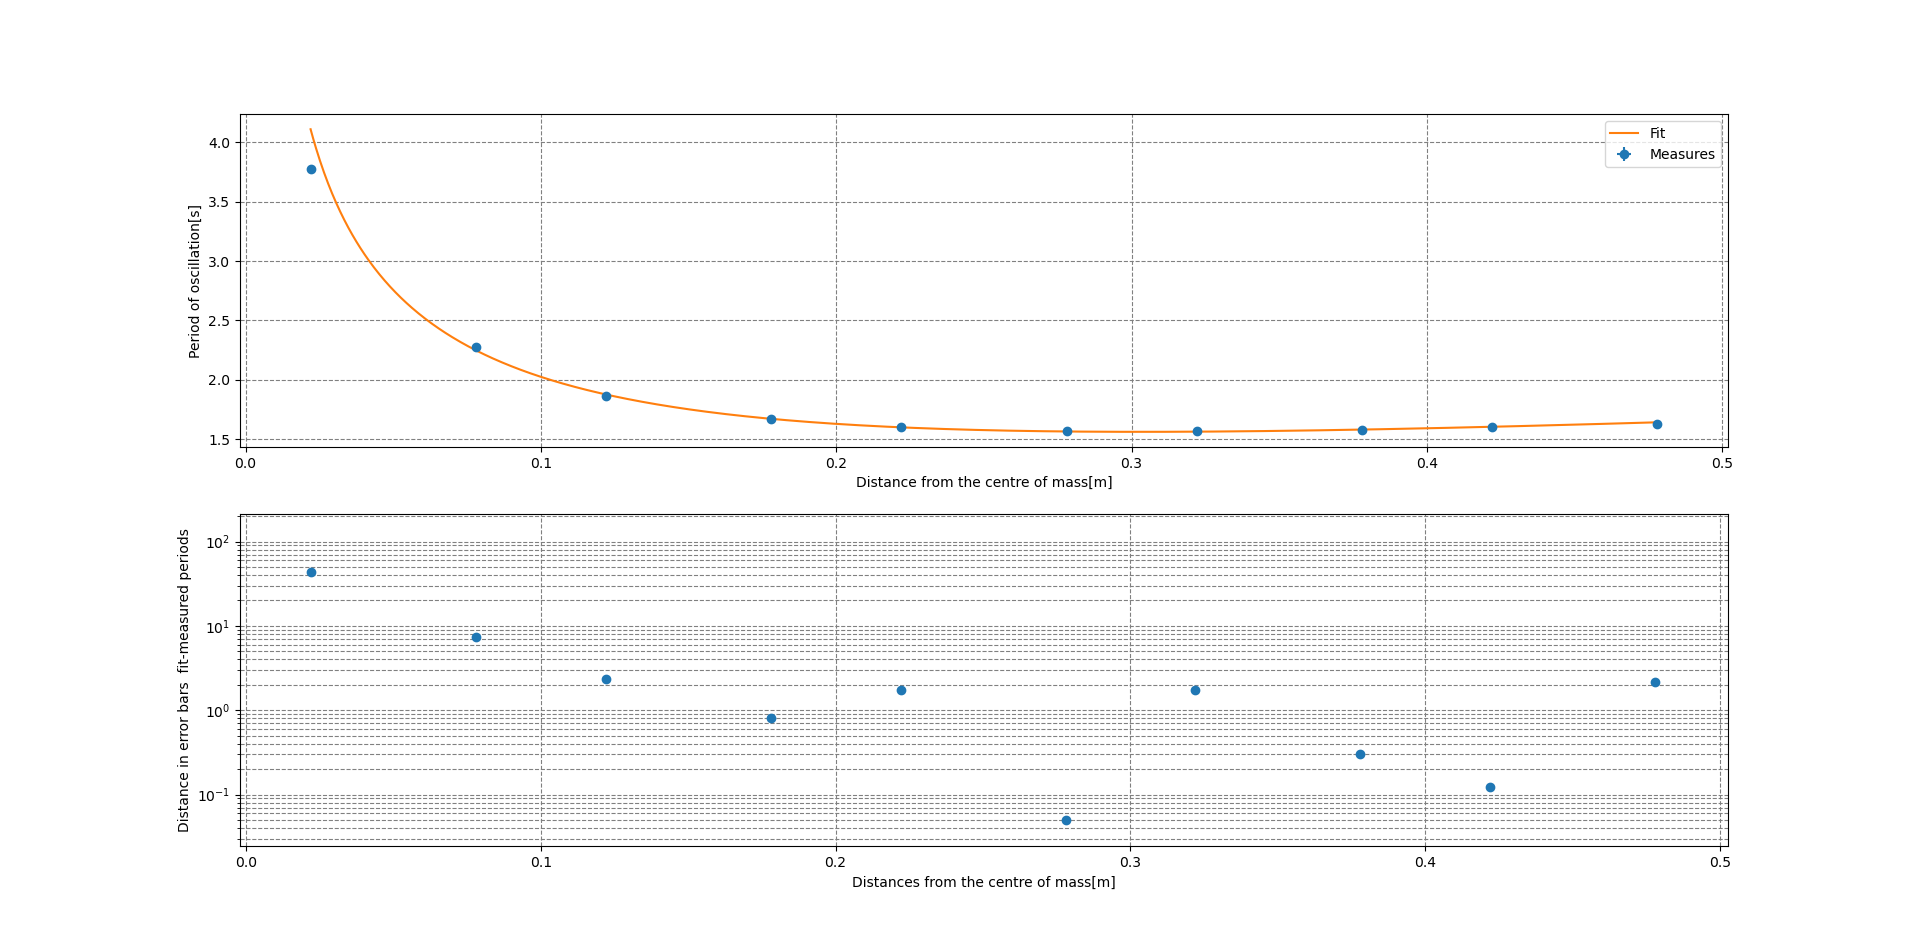
\includegraphics[width=20cm, height=15cm]{physicalpendulum_plots_1.0.png}}

\label{fig}
\end{figure}
Si osserva che la distanza in barre di errore tra la previsione della curva di best-fit e i dati presi sperimentalmente differiscono di più di 1 per quelle misure prese con la cerniera  sistemata vicino al centro di massa; mentre sono minori di 1 più il punto di sospensione si allontana dal centro di massa , eccetto che per un caso.
Il grafico degli scarti in carta semi-logaritmica suggerisce che la differenza tra fit e misure cresca esponenzialmente con l'avvicinarsi della distanza tra il punto di sospensione e quello del centro di massa a 0.
Questo fenomeno, contro le ipotesi iniziali discusse nel paragrafo "\textbf{Approssimazioni}", potrebbe essere causato dall'attrito della cerniera;tale ipotesi si concilierebbe anche col fatto che per punti di sospensione più distanti dal centro di massa questo fenomeno non è osservabile (il lavoro della forza di attrito sarebbe lo stesso, ma l'energia cinetica della rotazione è maggiore)  . 
Un'altra spiegazione potrebbe essere la seguente: le misure della distanza tra centro del foro e centro di massa, specialmente per il punto più vicino a quest ultimo, non sono state condotte correttamente.
Un'ulteriore causa potrebbe essere stata che l' ipotesi discussa nel paragrafo "\textbf{Asta omogenea}"  sia erronea.
\section{Conclusione}
Per quanto osservato dal grafico degli scarti, l'equazione (5) è un buon modello predittivo del periodo del pendolo eccetto che per distanze di sospensione troppo vicine al centro di massa.
\end{document}
